
%(BEGIN_QUESTION)
% Copyright 2011, Tony R. Kuphaldt, released under the Creative Commons Attribution License (v 1.0)
% This means you may do almost anything with this work of mine, so long as you give me proper credit

This is a PFD for a simple geothermal power plant, drawing a mixture of superheated steam and entrained minerals from a ``production well'' drilled deep into the earth, and injecting the condensed water and minerals into a second ``injection well'' to be re-heated by geothermal heat:

$$\includegraphics[width=15.5cm]{i00736x01.eps}$$

The HP throttle and turbine bypass control valves are split-ranged, to allow the turbine's power output to be adjusted according to how much electricity we wish to generate and not how much geothermal steam is available.  In essence, they act like the variable-pitch blades on wind turbines: when wind is low, they adjust for maximum power generation; when wind is high, they ``spill'' the excess wind to limit power generation at the generator's maximum limit.  Both valves are controlled by a single power controller monitoring power output of the generator.  

Determine a proper split-range for these two control valves, assuming we wish the HP throttle valve to be fail-closed and the bypass valve to be fail-open, and that the actuator operating range for each valve is 3-15 PSI:

% No blank lines allowed between lines of an \halign structure!
% I use comments (%) instead, so that TeX doesn't choke.

$$\vbox{\offinterlineskip
\halign{\strut
\vrule \quad\hfil # \ \hfil & 
\vrule \quad\hfil # \ \hfil & 
\vrule \quad\hfil # \ \hfil \vrule \cr
\noalign{\hrule}
%
% First row
{\bf Valve} & {\bf Fully shut at} & {\bf Fully open at} \cr
 & (PSI) & (PSI) \cr
%
\noalign{\hrule}
%
% Another row
HP throttle &  &  \cr
%
\noalign{\hrule}
%
% Another row
Turbine bypass &  &  \cr
%
\noalign{\hrule}
} % End of \halign 
}$$ % End of \vbox

Now suppose a maintenance mechanic accidently leaves a block valve shut in line with the turbine bypass valve.  Explain what effects this change will have on the entire power plant system (power output, level controls, pressures).

\vskip 20pt \vbox{\hrule \hbox{\strut \vrule{} {\bf Suggestions for Socratic discussion} \vrule} \hrule}

\begin{itemize}
\item{} If the block valve left shut by the mechanic is still {\it locked} and {\it tagged}, what do you think would be the proper procedure for un-locking and un-tagging the valve so that it may be opened?  Can anyone do this?  Why or why not?
\end{itemize}

\underbar{file i00736}
%(END_QUESTION)





%(BEGIN_ANSWER)

% No blank lines allowed between lines of an \halign structure!
% I use comments (%) instead, so that TeX doesn't choke.

$$\vbox{\offinterlineskip
\halign{\strut
\vrule \quad\hfil # \ \hfil & 
\vrule \quad\hfil # \ \hfil & 
\vrule \quad\hfil # \ \hfil \vrule \cr
\noalign{\hrule}
%
% First row
{\bf Valve} & {\bf Fully shut at} & {\bf Fully open at} \cr
 & (PSI) & (PSI) \cr
%
\noalign{\hrule}
%
% Another row
HP throttle & 3 PSI & 15 PSI \cr
%
\noalign{\hrule}
%
% Another row
Turbine bypass & 15 PSI & 3 PSI \cr
%
\noalign{\hrule}
} % End of \halign 
}$$ % End of \vbox

If the bypass line is blocked by a shut hand valve, the turbine power control system will still do its job to regulate output power, but other variables in the plant will certainly be affected!

%(END_ANSWER)





%(BEGIN_NOTES)

We aren't shown what sort of control system operates the HP separator vent valve, but presumably it is a pressure control system, which will have to open this valve if steam production exceeds the generator's power setpoint and there is no longer a bypass route around the turbine.

%INDEX% Process: geothermal power plant

%(END_NOTES)

